\section{Advent Nopele Olansi Damiahan Sihite (1174089)}
\subsection{Teori}
\begin{enumerate}
\item Definisi Kecerdasan buatan\\ 
Kecerdasan Buatan biasa disebut dengan istilah AI (Artificial Intelligence). Kecerdasan Buatan adalah salah satu bidang studi yang berhubungan dengan pemanfaatan mesin untuk memecahkan persoalan yang rumit dengan cara lebih manusiawi dan lebih bisa di pahami oleh manusia. Kecerdasan buatan makin canggih dengan kemampuan komputer dalam memperbarui pengetahuannya dengan banyaknya testing dan perkembangan target analisa. Untuk kecerdasan buatan ada banyak contoh dan jenisnya. Salah satu contoh yang paling terkenal dari Artificial Intelligence ialah Google Assistant. Google Assistant digunakan untuk kemudahan user dalam menemukan berbagai hal maupun penyetingan langsung terhadap smartphone yang digunakan dan masih banyak lagi.

\item Sejarah dan Perkembangan Kecerdasan Buatan
\begin{itemize}
\item Pada tahun 1943, pekerjaan pertama yang dikenal sebagai AI telah dilakukan oleh Warren McCulloch dan juga Walter Pits yang dinamakan sebagai artificial neurons
\item Pada tahun 1955, Allen Newell dan Herbert A. Simon membuat program kecerdasan buatan pertama yang dinamakan Logic Theorist
\item Pada tahun 1972, robot pertama dibuat di jepang dengan nama Wabot-1 dengan kecerdasan buatan
\item Pada tahun 1980, muncul bidang baru dari kecerdasan buatan yaitu Expert System yang membantu dalam pemberian keputusan
\item Tahun 1997, IBM deep blue mengalahkan juara catur dunia Gary Kasparov dan menjadi komputer pertama yang mengalahkannya
\item Tahub 2006, perusahaaan sudah mulai menerapkan kecerdasan buatan pada produknya seperti Netflix dan Twitter.
\item Tahun 2018,  	Project Debater dari IBM melakuakn debat tentang topik yang kompleks dan berakhir dengan hasil memuaskan
\end{itemize}

\item Definisi Supervised Learning\\
Supervised Learning adalah tugas pengumpulan data untuk menyimpulkan fungsi dari data pelatihan berlabel. Data pelatihan terdiri dari serangkaian contoh pelatihan. Dalam supervised learning, setiap contoh adalah pasangan yang terdiri dari objek input (biasanya vektor) dan nilai output yang diinginkan(juga disebut sinyal pengawasan super).

\item Klasifikasi Supervised Learning
\begin{itemize}
\item Klasifikasi adalah pembagian sesuatu menurut kelas-kelas ( class ). Menurut Ilmu Pengetahuan, Klasifikasi merupakan proses pengelompokkan benda berdasarkan ciriciri persamaan dan juga perbedaan. Dalam masalah klasifikasi, kami mencoba memprediksi sejumlah nilai terpisah. Label (y) umumnya datang dalam bentuk kategorikal dan mewakili sejumlah kelas. Dalam pembelajaran mesin dan statistik, klasifikasi adalah pendekatan pembelajaran yang diawasi di mana program komputer belajar dari input data yang diberikan kepadanya dan kemudian menggunakan pembelajaran ini untuk mengklasifikasikan pengamatan baru. Kumpulan data ini mungkin hanya bersifat dua kelas (seperti mengidentifikasi apakah orang tersebut berjenis kelamin laki-laki atau perempuan atau bahwa surat itu spam atau bukan-spam) atau mungkin juga multi-kelas. Beberapa contoh masalah klasifikasi adalah: pengenalan ucapan, pengenalan tulisan tangan, identifikasi metrik, klasifikasi dokumen dll.
\end{itemize}

\item Regresi dan Unsupervised Learning\\
Regresi adalah metode analisis statistik yang digunakan untuk melihat pengaruh antara dua ataupun lebih variabel. Regresi adalah membahas masalah ketika variabel output adalah nilai riil atau berkelanjutan, seperti ”gaji” atau ”berat”. Banyak model yang berbeda dapat digunakan makan, yang paling sederhana adalah regresi linier. Ia mencoba untuk menyesuaikan data dengan hyper-plane terbaik yang melewati poin.

Unsupervised Learning berbeda dengan Supervised Leraning. Perbedaannya ialah unsupervised learning tidak memiliki data latih, sehingga dari data yang ada kita mengelompokan data tersebut menjadi 2 ataupun 3 bagian dan seterusnya. Unsupervised Learning adalah pelatihan algoritma kecerdasan buatan (AI) menggunakan informasi yang tidak diklasifikasikan atau diberi label dan memungkinkan algoritma untuk bertindak atas informasi tersebut tanpa bimbingan. Algoritma Unsupervised Learning dapat melakukan tugas pemrosesan yang lebih kompleks daripada sistem pembelajaran yang diawasi

\item Dataset\\
Dataset adalah objek yang merepresentasikan data dan juga relasi yang ada di memory. Strukturnya mirip dengan data di database, namun bedanya dataset berisi koleksi dari data table dan data relation. mendapatkan data yang tepat berarti mengumpulkan atau mengidentifikasi data yang berkorelasi dengan hasil yang ingin Anda prediksi; yaitu data yang berisi sinyal tentang peristiwa yang Anda pedulikan. Data harus diselaraskan dengan masalah yang Anda coba selesaikan.

\item Training Set\\
Training Set adalah set digunakan oleh algoritma klassifikasi . Dapat dicontohkan dengan : decision tree, bayesian, neural network dll. Semuanya dapat digunakan untuk membentuk sebuah model classifier. Menjalankan pelatihan yang diatur melalui jaringan saraf mengajarkan pada net cara menimbang berbagai fitur, menyesuaikan koefisien berdasarkan kemungkinan mereka meminimalkan kesalahan dalam hasil Anda. Koefisien-koefisien tersebut, juga dikenal sebagai parameter, akan terkandung dalam tensor dan bersama-sama mereka disebut model, karena mereka mengkodekan model data yang mereka latih. Mereka adalah takeaways paling penting yang akan Anda dapatkan dari pelatihan jaringan saraf.

\item Testing Set\\
Testing Set adalah set yang digunakan untuk mengukur sejauh mana classifier berhasil melakukan klasifikasi dengan benar. Ini berfungsi sebagai meterai persetujuan, dan Anda tidak menggunakannya sampai akhir. Setelah Anda melatih dan mengoptimalkan data Anda, Anda menguji jaringan saraf Anda terhadap pengambilan sampel acak akhir ini. Hasil yang dihasilkannya harus memvalidasi bahwa jaring Anda secara akurat mengenali gambar, atau mengenalinya setidaknya [x] dari jumlah tersebut. Jika Anda tidak mendapatkan prediksi yang akurat, kembalilah ke set pelatihan, lihat hyperparameter yang Anda gunakan untuk menyetel jaringan, serta kualitas data Anda dan lihat teknik pra-pemrosesan Anda.
\end{enumerate}

\subsection{Instalasi}
\begin{enumerate}
	\item Instalasi Library scikit dari a naconda, mencoba kompilasi dan uji coba ambil contoh kode dan lihat variabel explorer
	\hfill\break
	\begin{figure}[H]
		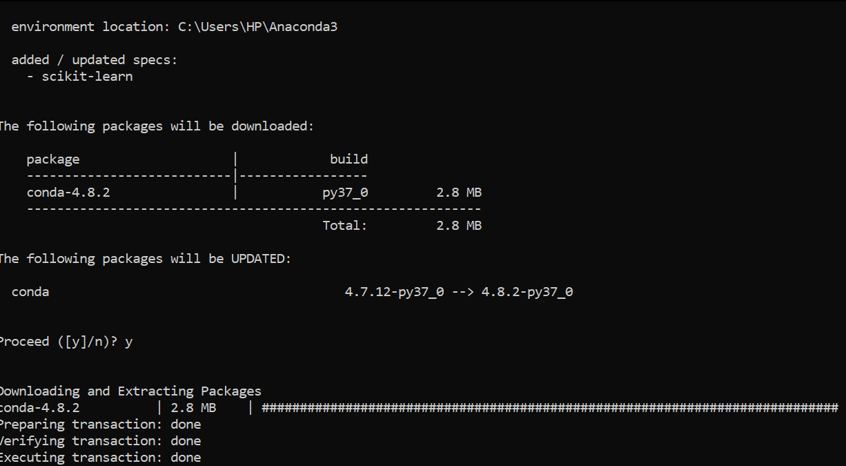
\includegraphics[width=4cm]{figures/1174089/1/1.png}
		\centering
		\caption{Instalasi Package Scikit Learn}
	\end{figure}
	\begin{figure}[H]
		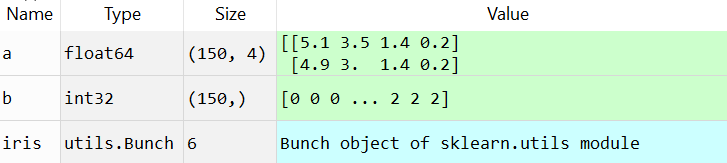
\includegraphics[width=4cm]{figures/1174089/1/2.png}
		\centering
		\caption{Isi Variabel Explorer}
	\end{figure}
	\item Mencoba Loading an example dataset, menjelaskan maksud dari tulisan tersebut dan mengartikan per baris
	\hfill\break
	\lstinputlisting[firstline=2, lastline=7]{src/1174089/1/1174089.py}
	\item Mencoba Learning and predicting, menjelaskan maksud dari tulisan tersebut dan mengartikan perbaris
	\hfill\break
	\lstinputlisting[firstline=9, lastline=28]{src/1174089/1/1174089.py}
	\item  Mencoba Model persistence, menjelaskan maksud dari tulisan tersebut dan mengartikan per baris
	\hfill\break
	\lstinputlisting[firstline=30, lastline=48]{src/1174089/1/1174089.py}
	\item Mencoba Conventions, menjelaskan maksud dari tulisan tersebut dan mengartikan per baris
	\hfill\break
	\lstinputlisting[firstline=50, lastline=72]{src/1174089/1/1174089.py}
\end{enumerate}

\subsection{Penanganan Error}
\begin{enumerate}
	\item ScreenShoot Error
	\begin{figure}[H]
		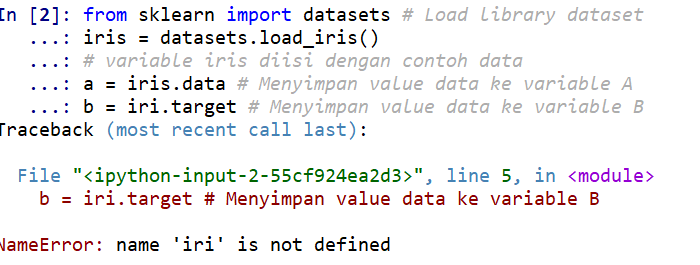
\includegraphics[width=4cm]{figures/1174089/1/error.PNG}
		\centering
		\caption{No Module Named Numpya}
	\end{figure}

	\item Tuliskan Kode Error dan Jenis Error
	\begin{itemize}
		\item ModuleNotFoundError
	\end{itemize}
	\item Cara Penangan Error
	\begin{itemize}
		\item ModuleNotFoundError
		\hfill\break
		Mengecek Typo dan menulis kembali library yang akan diimport
	\end{itemize}
\end{enumerate}

\subsection{Bukti Tidak Plagiat}
\begin{figure}[H]
	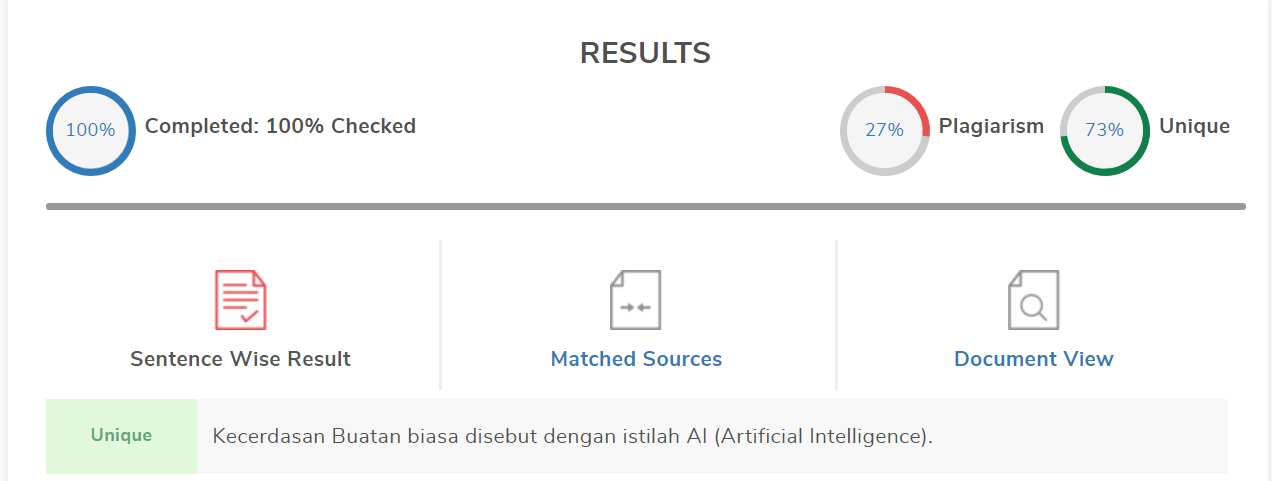
\includegraphics[width=4cm]{figures/1174089/1/plagiarism.PNG}
	\centering
	\caption{Bukti Tidak Melakukan Plagiat Chapter 1}
\end{figure}


